\section{Real World Languages}
\label{sec:real}

Our approach can be used to retrofit any language for which we
can achieve isolation with information flow control.
%
Unfortunately, controlling the external effects of a real-world
language, as to achieve isolation, is language-specific and varies
from one language to another.\footnote{
  Though we apply our framework to several real-world languages, it is
  conceivable that there are languages for which isolation cannot be
  easily achieved.
}
%
Indeed, even for a single language (e.g., JavaScript), how one
achieves isolation may vary according to the language runtime or
embedding (e.g., server and browser).
%

In this section, we describe several implementations and their
approaches to isolation.
%
In particular, we describe two JavaScript IFC implementations
building on the theoretical foundations of this work.
%
Then, we consider how our formalism could be applied to the C
programming language and connect it to a previous IFC system for
Haskell.
%



%% The goal of this section is to show the flexibility of the embedding in settings with
%% vastly different properties and discuss the
%% semantic gap that must be overcome to apply our formalism
%% to other systems.
%
%% Two of the systems we describe have been implemented: the Haskell
%% system~\cite{lio} and the COWL~\cite{swapi} system; we leave the
%% implementation of the IFC system for C to future work.


\subsection{JavaScript}
\label{sec:real:js}

JavaScript, as specified by
ECMAScript~\cite{ecma}, does not have any built-in
functionality for I/O.
%(we denote this language as |targetLangJS|).
%
For this language, which we denote by |targetLangJS|, the IFC system
|specLangJS roundrobinf| can be implemented by exposing IFC primitives
to JavaScript as part of the runtime, and running multiple instances
of the JavaScript virtual machine in separate OS-level threads.
%
Unfortunately, this becomes very costly when a system, such as a
server-side web application, relies on many tasks.
%
%% For instance, consider a server-side web application that
%% creates a new task for each HTTP request.  The overhead would
%% quickly become impractical.

Luckily, this issue is not unique to our work---browser layout engines
also rely on isolating code executing in separate iframes (e.g., according to the
same-origin policy).
%
Since creating an OS thread for each iframe is expensive, both
the V8 and SpiderMonkey JavaScript engines provide means for running
JavaScript code in isolation within a single OS thread,
on disjoint sub-heaps.
%
In V8, this unit of isolation is called a \emph{context}; in
SpiderMonkey, it is called a \emph{compartment}.
%
(We will use these terms interchangeably.)
%
Each context is associated with a global object, which, by
default, implements the JavaScript standard library (e.g.,
\verb|Object|, \verb|Array|, etc.).
%
Naturally, we adopt contexts to implement our notion of tasks.


When JavaScript is embedded in browser layout engines,
or in server-side platforms such as Node.js,
additional APIs such as the Document Object Model (DOM) or the file
system get exposed as part of the runtime system.
These features are exposed by extending the global object, just like
the standard library.  For this reason, it is easy to modify
these systems to forbid external effects when implementing
an IFC system, ensuring that important effects can be reintroduced in a safe manner.



\begin{figure}[t]
\centerline{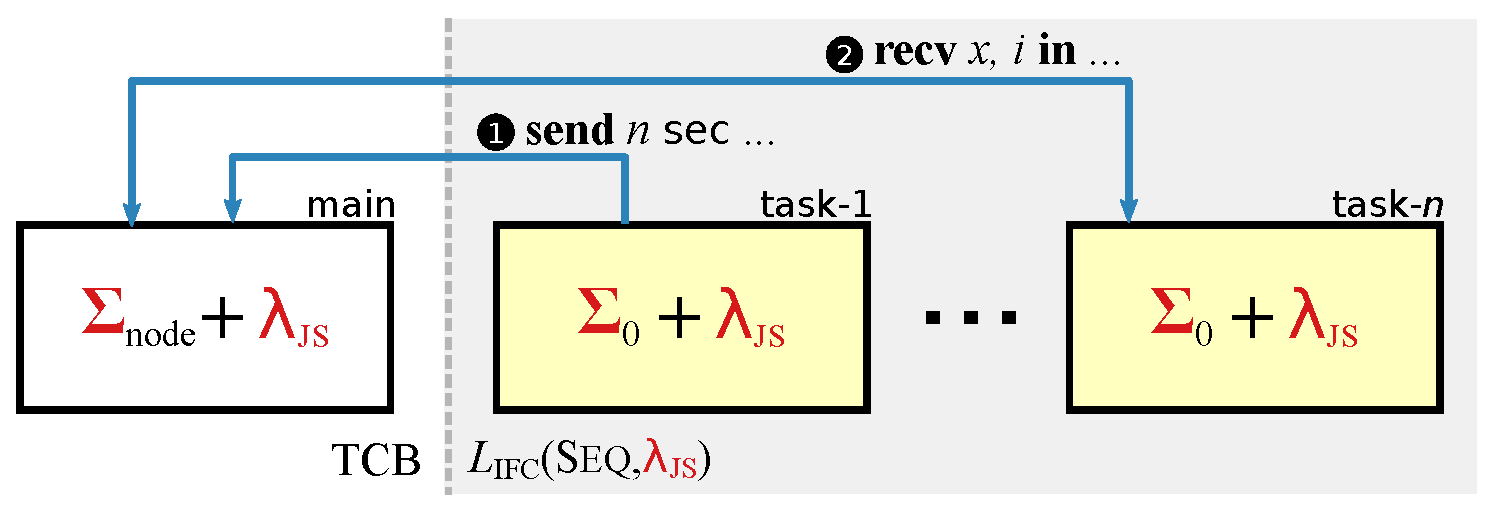
\includegraphics[width=0.7\columnwidth]{figs/node}}
\caption{\label{fig:node}
This example shows how our trusted monitor (left) is used to mediate
communication between two tasks for which IFC is enforced (right).}
\end{figure}
%
\paragraph{Server-side IFC for Node.js:}
We have implemented |specLangJS seqf| for Node.js in the form of a
library, without modifying Node.js or the V8 JavaScript engine.
%
Our implementation\footnote{Available at \codelink{}.} provides a
library for creating new tasks, i.e., contexts whose global object
only contains the standard JavaScript library and our IFC primitives
(e.g., |send| and |sandbox|).
%
When mapped to our formal treatment, |sandbox| is defined with |ap
klone tS = tS0|, where |tS0| is the global object corresponding to the
standard JavaScript library and our IFC primitives.
%
%These tasks can communicate and create new tasks, in turn.
%
These IFC operations are mediated by the trusted library code (executing
as the main Node.js context), which tracks the state (current label, messages,
etc.) of each task.  An example for |send|/|recv| is shown in
Fig.~\ref{fig:node}.
%While V8 provides a means for sharing any object between contexts (used
%by same-origin contexts in Blink),
Our system conservatively restricts the kinds of messages that can be
exchanged, via |send| (and |sandbox|), to string values.
%
%
In our formalization, this amounts to restricting the IFC language rule
for |send| in the following way:
%{
\newcommand{\str}{"string"}
%format tOf (e) = "\texttt{typeOf}("e")\texttt{ === \str}"
%format ttrue = "\texttt{true}"
\begin{mathpar}
\inferrule[JS-send]
{
|il canFlowTo il'|\\
|iS(id') = Q|\\
|iS' = iS [ mapsto id' (il', id,  iv) , Q ]|\\
|ie = IT te|\\
|conf tS (tOf te) -> conf tS ttrue|
}
{|
iconf iS (fullconf id il tS (iniEi (send id' il' iv)), ldots)
.->
iS'; sched step (fullconf id il tS (iniEi unit), ldots)
|}
\end{mathpar}
%}
%
Of course, we provide a convenience library which marshals JSON
objects to/from strings.
%
We remark that this is not unlike existing message-passing JavaScript
APIs, e.g., \texttt{postMessage}, which impose similar restrictions as
to avoid sharing references between concurrent code.

While the described system implements |specLangJS seqf|, applications
typically require access to libraries (e.g., the file system library
\textsf{fs}) that have external effects.
%
Exposing the Node.js APIs directly to sandboxed tasks is unsafe.
Instead, we implement libraries (like a labeled version of \textsf{fs}) as
message exchanges between the sandboxed tasks (e.g., \textsf{task-1}
in Fig.~\ref{fig:node}) and the main Node.js task that implements
the IFC monitor.
%
While this is safer than simply wrapping unsafe objects, which can
potentially be exploited to access objects outside the context (e.g.,
as seen with
\ifextended
ADSafe, FBJS, and Caja~\cite{taly2011automated, maffeis2010object, maffeis2009language}),
\else
ADSafe~\cite{taly2011automated}),
\fi
adding features such as the
\textsf{fs} requires the code in the main task to ensures that labels
are properly propagated and enforced.
%
Unfortunately, while imposing such a proof burden
is undesirable, this also has to be expected:
different language environments expose different libraries for
handling external I/O, and the correct treatment of external effects
is application specific.
%
%% For instance, in the case of Node.js, how labels interact with the
%% file system may even vary according to the application (e.g.,
%% in the IFC system Hails~\cite{hails}, labels are not persisted).
%
%While we can extend our formalism to model a particular interface to
%the file system, HTTP client, etc. the utility of this formalization is
%unclear and left to future work.
%
We do not extend our formalism to account for the  particular
interface to the file system, HTTP client, etc., as this is
specific to the Node.js implementation and does not generalize
to other systems.


\paragraph{Client-side IFC:}
This work provides the formal basis for the core part of the COWL
client-side JavaScript IFC system~\cite{swapi}.
%
Like our Node.js implementation, COWL takes a coarse-grained approach
to providing IFC for JavaScript programs.
%
%Unlike our implementation,
However, COWL's IFC monitor is implemented in
the browser layout engine instead (though still leaving the JavaScript engine
unmodified).

Furthermore, COWL repurposes existing contexts (e.g., iframes and
pages) as IFC tasks, only imposing additional constraints on how they
communicate.
%
As with Node.js, at its core, the global object of a COWL task
should only contain the standard JavaScript libraries and
\texttt{postMessage}, whose semantics are modeled by our
\textsc{JS-send} rule.
%
However, existing contexts have objects such as the DOM, which
require COWL to restrict a task's external effects.
%
To this end, COWL mediates any communication (even via the DOM) at
the context boundary. %by COWL.

Simply disallowing all the external effects is overly-restricting for
real-world applications (e.g., pages typically load images, perform
network requests, etc.).
%
In this light, COWL allows safe network communication by associating an
implicit label with remote hosts (a host's label corresponds to
its origin).
%
In turn, when a task performs a request, COWL's IFC monitor
ensures that the task label can flow to the remote origin label.
%
While the external effects of COWL can be formally modeled, we do not
model them in our formalism, %more general framework,
since, like for the
Node.js case, they are specific to this system.
%
%Indeed, even the labeled HTTP client in  Node.js and COWL differ, even
%though they're both JavaScript systems, simply because of the
%differing environments.



\subsection{Haskell}
\label{sec:real:hs}
Our work borrows ideas from the LIO Haskell coarse-grained IFC
system~\cite{lio, stefan:addressing-covert}.
%
LIO relies on Haskell's type system and monadic encoding of
effects to achieve isolation and define the IFC sub-language.
%
Specifically, LIO provides the \verb|LIO| monad as a way of restricting
(almost all) side-effects.
%
In the context of our framework, LIO can be understood as follows: the
\emph{pure subset} of Haskell is the target language, while the
monadic subset of Haskell, operating in the \verb|LIO| monad, is the
IFC language.

%Indeed, by rephrasing LIO in terms of our framework, we simplified
%LIO's treatment of exceptions.
%
Unlike our proposal, LIO originally associated labels with exceptions, in a
similar style to fine-grained
systems~\cite{stefan:2012:arxiv-flexible, Hritcu:2013:YIB:2497621.2498098}.
%
In addition to being overly complex, the interaction of exceptions
with clearance (which sets an upper bound on the floating label, see
\appref{sec:clearance}) was incorrect: the clearance
was restored to the clearance at point of the catch.
%
Furthermore, pure exceptions (e.g., divide by zero) always percolated to
trusted code, effectively allowing for denial of service attacks.
%
The insights gained when viewing coarse-grained IFC as presented in this
paper led to a much cleaner, simpler treatment of exceptions,
which has now been adopted by LIO.
%By using isolated tasks, and thus treating the current label (and
%clearance) as global, the underlying Haskell exception system can be
%used directly: exceptional control flow does not affect IFC.






\subsection{C}
\label{sec:real:c}
%
C programs are able to execute arbitrary (machine) code, access
arbitrary memory, and perform arbitrary system calls.
%
Thus, the confinement of C programs must be imposed by the underlying OS
and hardware.
%
For instance, our notion of isolation can be achieved using Dune's
hardware protection mechanisms~\cite{Belay:2012:DSU:2387880.2387913},
similar to 
Wedge~\cite{Belay:2012:DSU:2387880.2387913,
Bittau:2008:WSA:1387589.1387611}, but using an information flow control
policy.
%
Using page tables, a (trusted) IFC runtime could ensure that each task,
implemented as a lightweight process, can only access the memory it
allocates---tasks do not have access to any shared memory.
%
In addition, ring protection could be used to intercept system
calls performed by
a task and only permit those corresponding to our IFC language (such as
|getLabel| or |send|).
%
Dune's hardware protection mechanism would allow us to provide a concrete
implementation that is efficient and relatively simple to reason
about, but other sandboxing mechanisms could be used in place of Dune.

In this setting, the combined language of Section~\ref{sec:retrofit}
can be interpreted in the following way: calling from the target
language to the IFC language corresponds to invoking a system call.
%
Creating a new task with the |sandbox| system call corresponds to
\emph{forking} a process.  Using page tables, we can ensure that
there will be no shared memory
(effectively
defining |ap klone tS
= tS0|, where |tS0| is the set of pages necessary to bootstrap a
lightweight process).
%
Similarly, control over page tables and protection bits allows us to
define a |send| system call that copies pages to our
(trusted) runtime queue; and, correspondingly, a |recv| that copies
the pages from the runtime queue to the (untrusted) receiver.
%
Since C is not memory safe, conditions on these system calls are
meaningless.
%
We leave the implementation of this IFC system for C as future work.
